\documentclass[10pt,a4paper]{article}

\newcommand{\cvRolle}{Senior Cloud Infrastructure \& DevOps Engineer}
\newcommand{\cvSubheader}{CI/CD Automation $\cdot$ Release Optimization $\cdot$ Platform Engineering Specialist}

% ==========================================
% SETTINGS.TEX - ZENTRALE KONFIGURATION
% ==========================================
\usepackage[utf8]{inputenc}
\usepackage[T1]{fontenc}
\usepackage[american]{babel}
\usepackage[top=1.8cm, bottom=1.8cm, left=1.8cm, right=1.8cm]{geometry}
\usepackage{xcolor}
\usepackage{hyperref}
\usepackage{enumitem}
\usepackage{graphicx}
\usepackage{calc}
\usepackage{charter}
\usepackage{microtype}
\usepackage{etoolbox}

% --- DESIGN FARBEN ---
\definecolor{primary}{RGB}{15, 23, 42}      % Deep Slate / Tech Dark
\definecolor{accent}{RGB}{37, 99, 235}     % MP Blue Accent
\definecolor{textgray}{RGB}{51, 65, 85}    % Charcoal Body Text

% --- PERMANENTE ABSENDER-DATEN ---
\newcommand{\meinName}{Markus Gruber, M.Sc.}
\newcommand{\meineStrasse}{Maximilianstraße 55 Stg. B 20}
\newcommand{\meinOrt}{3100 St. Pölten}
\newcommand{\meineEmail}{Markus.Gruber4@gmx.net}
\newcommand{\meineTel}{+43 650 5871145}
\newcommand{\meinLinkedin}{https://www.linkedin.com/in/markus-gruber-70851428/}
\newcommand{\meinGithub}{https://github.com/CodeByMaxx}

% --- ROLLEN-DEFAULTS ---
\providecommand{\cvRolle}{}
\renewcommand{\cvRolle}{AI & Automation Engineer -- M&A Deal Automation}
\providecommand{\cvSubheader}{}
\renewcommand{\cvSubheader}{Python \cdot LLM APIs (OpenAI, Anthropic) \cdot Financial Data Pipelines \cdot Agent Workflows \cdot RAG}

% --- EMPFÄNGER-DATEN ---
\newcommand{\firmenName}{MP Corporate Finance}
\newcommand{\ansprechPartner}{Katharina Schwarzl-Moser (HR Manager)}
\newcommand{\firmenStrasse}{Wien, Österreich}
\newcommand{\firmenOrt}{Wien, Österreich}

% --- INTELLIGENTE ADRESS-AUSGABE (Verhindert doppelte Zeilen, wenn Straße == Ort) ---
\newcommand{\firmenAdresse}{%
    \def\tempStrasse{Wien, Österreich}%
    \def\tempOrt{Wien, Österreich}%
    \ifx\tempStrasse\tempOrt
        \tempOrt%
    \else
        Wien, Österreich \\[0.15em] Wien, Österreich%
    \fi
}

\newcommand{\stellenTitel}{AI & Automation Engineer (f/m/x)}
\newcommand{\referenzNummer}{}

\newcommand{\anrede}{Dear Ms. Schwarzl-Moser,}
\newcommand{\firmenHighlight}{MP Corporate Finance is one of Europe's leading mid-market M&A boutiques, where your AI tools will be deployed on live cross-border transactions from day one.}

% --- HEADER BEFEHL ---
\newcommand{\cvHeader}{%
\begin{center}
    {\Huge\bfseries\color{primary} \meinName}\\[0.1cm]
    {\large\bfseries \cvRolle}\\[0.05cm]
    {\color{accent}\textbf{\cvSubheader}}\\[0.1cm]
    {\small \meinOrt, Austria \quad$\cdot$\quad \meineTel \quad$\cdot$\quad \href{mailto:\meineEmail}{\meineEmail} \quad$\cdot$\quad \href{\meinLinkedin}{LinkedIn} \quad$\cdot$\quad \href{\meinGithub}{GitHub}}
\end{center}
\vspace{0.1cm}
}

% --- BEFEHLE FÜR LEBENSLÄUFE & ANSCHREIBEN ---
\newcommand{\cvsection}[1]{%
    \vspace{0.25cm}%
    {\Large\bfseries\color{primary} #1}\par%
    \vspace{-0.1cm}{\color{primary}\rule{\textwidth}{0.8pt}}\par%
    \vspace{0.15cm}%
}

\newcommand{\daterange}[2]{\hfill{\small #1 -- #2}}

% --- ENGINEERING APPROACH & MINDSET DEFINITION ---
\newcommand{\engineeringApproach}{%
    \cvsection{Engineering Approach \& Mindset}%
    \begin{itemize}[leftmargin=*, itemsep=2pt]%
        \item \textbf{Systematic Problem Solving:} First-principles analytical approach to systematic debugging and stability optimization.%
        \item \textbf{Quality & Efficiency Focus:} Pragmatic engineering mindset balancing rapid deployment with long-term maintainability and high performance.%
        \item \textbf{Cross-Functional Integration:} Acts as the technical glue bridging development, QA, and architecture.%
    \end{itemize}%
}

% --- HYPERREF SETUP ---
\hypersetup{
    colorlinks=true,
    linkcolor=primary,
    urlcolor=primary,
    pdfauthor={\meinName},
    pdftitle={Application Documents - \meinName}
}


\pagestyle{empty}

\begin{document}

\setlength{\parindent}{0pt}
\setlist[itemize]{leftmargin=1.5em, itemsep=0.15em, topsep=0.15em}

\cvHeader

\cvsection{Professional Profile}

% --- BILD LINKS, TEXT RECHTS UNTER DER ÜBERSCHRIFT ---
\begin{minipage}[t]{0.22\textwidth}
    \vspace{0pt}
    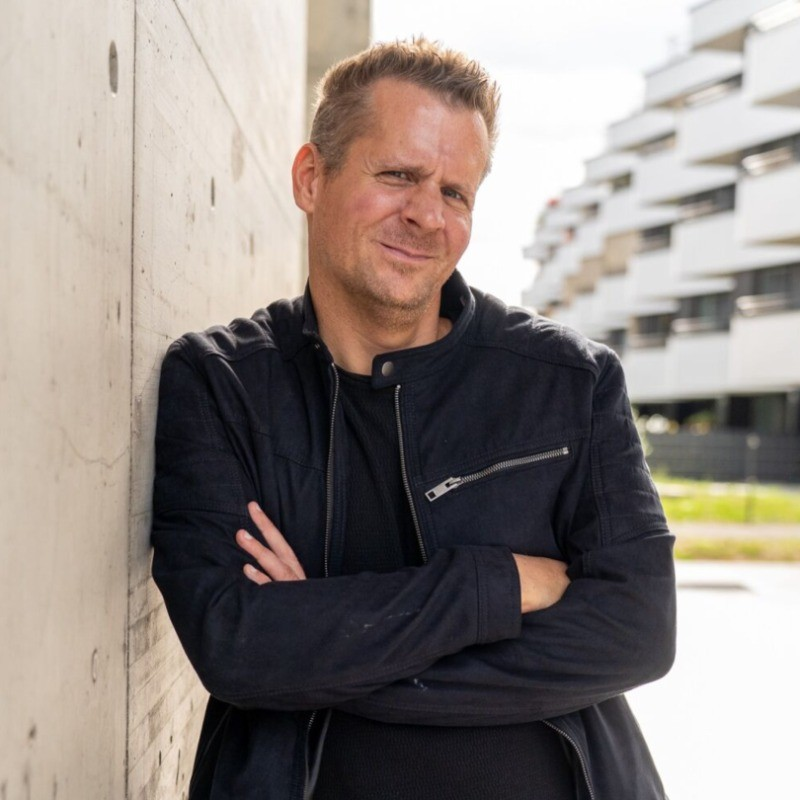
\includegraphics[width=\linewidth, keepaspectratio]{profil.jpeg}
\end{minipage}
\hfill
\begin{minipage}[t]{0.75\textwidth}
    \vspace{0pt}
    Senior Cloud Infrastructure \& DevOps Engineer with 9+ years of experience automating build pipelines, optimizing container workloads, and maintaining high-availability software platforms. Holds an M.Sc. in Scientific Computing.\\\\[0.1cm]
    Specializes in reducing release cycle times, establishing robust telemetry/monitoring, and unifying development and ops workflows through infrastructure as code and automated release verification.
\end{minipage}

\vspace{0.3cm}

\cvsection{Engineering Profile}

\colorbox{primary!10}{%
\parbox{\dimexpr\textwidth-2\fboxsep\relax}{%
    \vspace{0.10cm}
    \centering
    {\bfseries\color{primary} TECHNICAL FOUNDATION \& SYSTEM DOMAINS\par}
    \vspace{0.08cm}

    \begin{minipage}[t]{0.31\linewidth}
        \raggedright
        \textbf{\color{primary}DevOps \& CI/CD}\par
        GitLab CI/CD, Azure DevOps\\
        Automated Release Testing\\
        Pipeline Optimization \& Build Infra
    \end{minipage}
    \hfill
    \begin{minipage}[t]{0.31\linewidth}
        \raggedright
        \textbf{\color{primary}Cloud \& Containers}\par
        Docker \& Container Workloads\\
        Kubernetes / OpenShift\\
        AWS (S3, EC2, RDS) \& Azure
    \end{minipage}
    \hfill
    \begin{minipage}[t]{0.31\linewidth}
        \raggedright
        \textbf{\color{primary}Systems \& Scripting}\par
        Linux Administration (Ubuntu/Debian)\\
        Python, Bash, C++ System Integration\\
        Telemetry, Logging \& Monitoring
    \end{minipage}

    \vspace{0.08cm}
}%
}

\vspace{0.20cm}
\textbf{\color{primary}CORE TECHNICAL SPECIALIZATION -- PLATFORM ENGINEERING}
\begin{itemize}
    \item \textbf{CI/CD Pipeline Automation:} Designing scalable build and deployment pipelines, reducing release testing overhead and accelerating time-to-market.
    \item \textbf{Containerization \& Cloud Operations:} Managing Docker container orchestration, environment standardization, and cross-platform infrastructure stability.
    \item \textbf{System Profiling \& Performance Optimization:} Root-cause analysis of build bottlenecks, telemetry tracking, and automating release verification suites.
\end{itemize}

\cvsection{Professional Experience}

\textbf{Mindbreeze GmbH -- Quality / DevOps Engineer} \daterange{09/2022}{07/2026}\\
\textit{Python, Bash, Docker, Azure DevOps, Linux, Telemetry \& Performance Profiling \quad|\quad Team: 6 Engineers}
\begin{itemize}
    \item Engineered Python/Bash automation frameworks, reducing release verification duration from 10 working days down to 3 working days.
    \item Managed Docker container builds and Linux test infrastructure for high-throughput enterprise search backends.
    \item Deployed automated integration and regression test suites to monitor live platform performance and catch release defects early.
    \item Primary technical troubleshooter during release phases, resolving system bottlenecks and performance degradations in live environments.
\end{itemize}

\vspace{0.15cm}
\textbf{Untis GmbH -- Software Engineer (C++)} \daterange{02/2022}{06/2022}\\
\textit{C++, System Refactoring, Build Environment, Windows/Linux \quad|\quad Team: 10 Engineers}
\begin{itemize}
    \item Refactored core application modules, eliminated legacy technical debt, and streamlined Visual Studio build configurations.
\end{itemize}

\vspace{0.15cm}
\textbf{logi.cals -- Embedded Software Engineer (C/C++)} \daterange{02/2021}{01/2022}\\
\textit{C, C++, CI/CD Verification, Safety-Critical Architectures, Embedded Systems \quad|\quad Team: 6 Engineers}
\begin{itemize}
    \item Integrated automated test verification into build pipelines for safety-critical execution runtimes across hardware platforms.
\end{itemize}

\vspace{0.15cm}
\textbf{EYYES -- Software Engineer (C++/Python)} \daterange{04/2017}{12/2020}\\
\textit{Linux, Docker, CUDA, Edge Infrastructure, Real-Time Pipelines \quad|\quad Team: 8 Engineers}
\begin{itemize}
    \item Maintained deployment pipelines and edge device execution infrastructure for embedded GPU vision hardware.
    \item Automated hardware-near benchmarking and test routines, achieving 99.99\% classification precision in production environments.
\end{itemize}

\cvsection{Selected Software Projects}

\begin{itemize}
    \item \textbf{AWS Cloud Deep Learning Pipeline:} MLOps pipeline with automated ingestion and PyTorch inference (\href{\meinGithub}{GitHub}).\\
    \textit{Tech: AWS, Python, PyTorch, MLOps, CI/CD}
    \item \textbf{Azure AI Document Analyzer \& RAG Infra:} RAG processing backend deployed on Azure with vector databases (\href{\meinGithub}{GitHub}).\\
    \textit{Tech: Azure, Docker, Python, RAG, REST APIs}
\end{itemize}

\cvsection{Technical Skills}

\textbf{DevOps \& Tooling:} GitLab CI/CD, Azure DevOps, GitHub Actions, Docker, Kubernetes/OpenShift, Git, Telemetry, Linux Administration.\\[0.05em]
\textbf{Scripting \& Systems:} Python, Bash, Modern C++, C, SQL, Parallel Algorithms, Multithreading.\\[0.05em]
\textbf{Cloud Platform:} Amazon AWS (S3, RDS, EC2), Microsoft Azure, Linux (Ubuntu/Debian), Microservices, REST APIs.\\[0.05em]
\textbf{Data \& Infrastructure:} PostgreSQL, DuckDB, Apache Superset, CUDA, OpenCL.

\cvsection{Education}

\textbf{M.Sc. Scientific Computing} -- University of Vienna \daterange{10/2013}{06/2017}\\
\textit{Thesis: Silent Data Corruption in FT-GMRES (\href{https://utheses.univie.ac.at/detail/40917/}{Link}, Advisor: Prof. Dr. W. Gansterer).}

\vspace{0.1cm}
\textbf{B.Sc. Industrial Simulation} -- FH St. Pölten \daterange{09/2010}{06/2013}\\
\textit{Thesis: Simulation of Nanocomposite Materials (\href{\meinGithub}{Link}, Advisor: Prof. Dr. T. Schrefl).}

\engineeringApproach

\cvsection{Languages \& Work Status}

\textbf{German:} Native (C2) \quad$\cdot$\quad \textbf{English:} Full Professional Proficiency (C1/C2) \quad$\cdot$\quad \textbf{Work Permit:} EU Citizen / Austria

\end{document}
